\documentclass[border=0pt,tikz]{standalone}
% Nature Portfolio / Scientific Data shared TikZ style for IRexp figures.
% Width: 183 mm double-column. Typography: Helvetica-class (phv).
\RequirePackage{tikz}
\RequirePackage{pgfplots}
\RequirePackage{xcolor}
\RequirePackage{helvet}
\IfFileExists{sansmathfonts.sty}{\RequirePackage{sansmathfonts}}{}
\renewcommand{\familydefault}{\sfdefault}
\pgfplotsset{compat=1.18}
\usetikzlibrary{
  arrows.meta,calc,positioning,fit,shapes.geometric,shapes.misc,
  backgrounds,shadows.blur,patterns,decorations.pathreplacing
}

% ---- Paul Tol / NMRexp-matched palette ----
\definecolor{nmrBlue}{HTML}{4A7EBB}
\definecolor{nmrBlueDark}{HTML}{2E5F8F}
\definecolor{nmrBlueLight}{HTML}{A8C8E8}
\definecolor{nmrPeach}{HTML}{E8B48C}
\definecolor{nmrNavy}{HTML}{1B3D5C}
\definecolor{nmrRed}{HTML}{C44E52}
\definecolor{nmrGreen}{HTML}{3D8B5E}
\definecolor{nmrOrange}{HTML}{D97B32}
\definecolor{ink}{HTML}{1A1A1A}
\definecolor{muted}{HTML}{7A7F85}
\definecolor{note}{HTML}{5C636A}
\definecolor{faint}{HTML}{E8EAEC}
\definecolor{ghost}{HTML}{C5C9CD}
\definecolor{tintBlue}{HTML}{EEF3F8}
\definecolor{tintGreen}{HTML}{EAF4EE}

\newcommand{\NatureFont}{\fontfamily{phv}\selectfont}
\newcommand{\PanelLabel}[1]{%
  {\NatureFont\bfseries\fontsize{8}{9.6}\selectfont #1}%
}
\newcommand{\FigBody}{\NatureFont\fontsize{7}{8.4}\selectfont}
\newcommand{\FigSmall}{\NatureFont\fontsize{5.5}{6.6}\selectfont}
\newcommand{\FigAxis}{\NatureFont\fontsize{7}{8.4}\selectfont}

\tikzset{
  nature arrow/.style={
    -{Latex[length=1.6mm,width=1.3mm]},
    line width=0.55pt, ink
  },
  nature arrow grey/.style={
    -{Latex[length=1.6mm,width=1.3mm]},
    line width=0.5pt, note
  },
  stage card/.style={
    draw=nmrBlueDark, line width=0.7pt, rounded corners=2.2pt,
    fill=white, inner sep=3pt, align=center, font=\FigBody
  },
  stage header/.style={
    fill=nmrBlueDark, text=white, font=\FigBody\bfseries,
    rounded corners=2.2pt, inner sep=2.5pt, align=center
  },
  soft card/.style={
    draw=ghost, line width=0.55pt, rounded corners=2.2pt,
    fill=white, inner sep=3.5pt, align=left, font=\FigBody
  },
}

\pgfplotsset{
  nature axis/.style={
    tick label style={font=\FigSmall, /pgf/number format/assume math mode},
    label style={font=\FigAxis\bfseries},
    title style={font=\FigBody\bfseries, color=ink},
    axis line style={ink, line width=0.5pt},
    tick style={ink, line width=0.45pt},
    major grid style={faint, line width=0.35pt},
    axis x line=bottom,
    axis y line=left,
    enlarge x limits=false,
    clip=false,
  },
  nature hbar/.style={
    nature axis,
    xbar,
    bar width=7pt,
    y=data,
    nodes near coords,
    every node near coord/.append style={
      font=\FigSmall, ink, anchor=west, /pgf/number format/fixed,
      /pgf/number format/1000 sep={,}
    },
    xtick=\empty,
    axis x line=none,
    y axis line style={ink, line width=0.55pt},
    ytick style={draw=none},
    y tick label style={font=\FigBody, ink, anchor=east},
    grid=major x,
    xmin=0,
  },
}

\usepackage[T1]{fontenc}
\usepackage{textcomp}

\begin{document}
\NatureFont
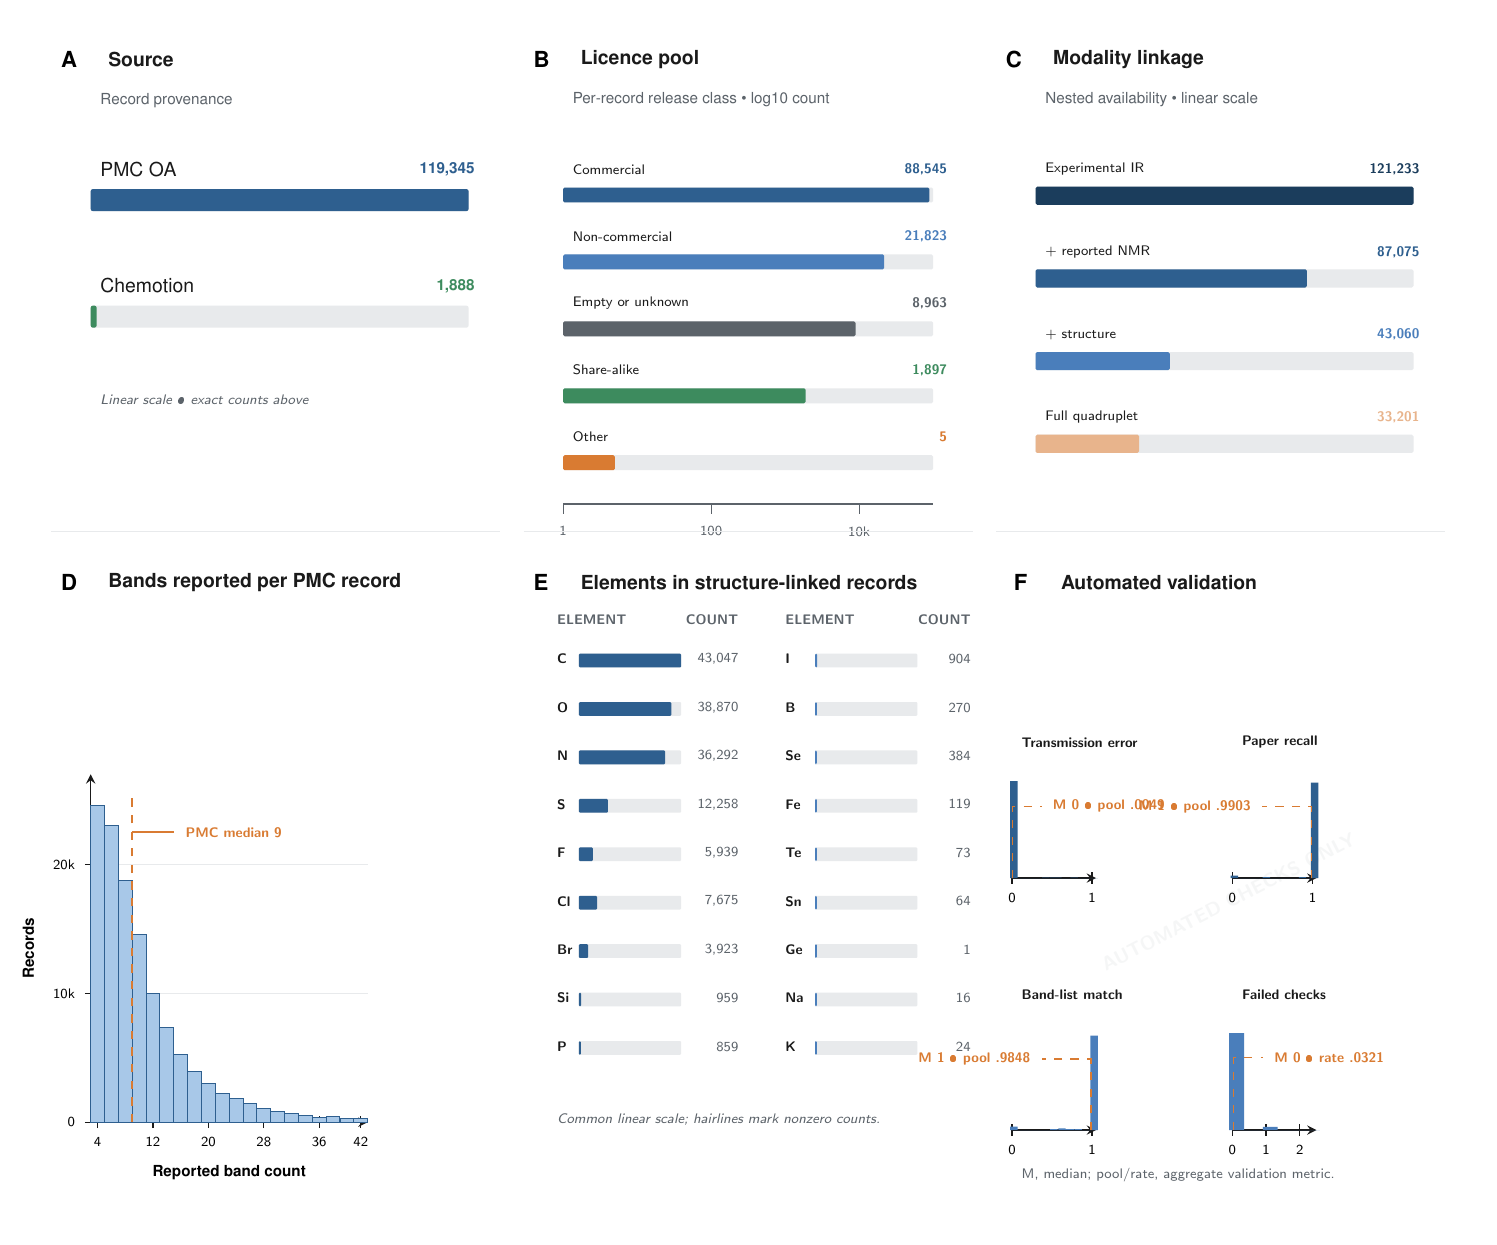
\begin{tikzpicture}[x=1mm,y=1mm]
  \path[use as bounding box] (0,0) rectangle (183,151);
  \fill[white] (0,0) rectangle (183,151);

  % ==========================================================================
  % A — Source
  \node[anchor=west] at (3,147) {\PanelLabel{A}};
  \node[anchor=west,font=\FigBody\bfseries,text=ink] at (9,147) {Source};
  \node[anchor=west,font=\FigSmall,text=note] at (8,141.8) {Record provenance};

  \node[anchor=west,font=\FigBody,text=ink] at (8,133) {PMC OA};
  \node[anchor=east,font=\FigSmall\bfseries,text=nmrBlueDark] at (58,133) {119,345};
  \fill[faint,rounded corners=.8pt] (8,127.7) rectangle (56,130.5);
  \fill[nmrBlueDark,rounded corners=.8pt] (8,127.7) rectangle (56,130.5);

  \node[anchor=west,font=\FigBody,text=ink] at (8,118.2) {Chemotion};
  \node[anchor=east,font=\FigSmall\bfseries,text=nmrGreen] at (58,118.2) {1,888};
  \fill[faint,rounded corners=.8pt] (8,112.9) rectangle (56,115.7);
  \fill[nmrGreen,rounded corners=.8pt] (8,112.9) rectangle +(.76,2.8);

  \node[anchor=west,font=\fontsize{5}{6}\selectfont\itshape,text=note]
    at (8,103.8) {Linear scale \textbullet\ exact counts above};
  \draw[faint,line width=.45pt] (3,87) -- (60,87);

  % ==========================================================================
  % B — Licence pool (log forest bars)
  \node[anchor=west] at (63,147) {\PanelLabel{B}};
  \node[anchor=west,font=\FigBody\bfseries,text=ink] at (69,147) {Licence pool};
  \node[anchor=west,font=\FigSmall,text=note] at (68,141.8) {Per-record release class \textbullet\ log10 count};

  \foreach \lab/\val/\yy/\col/\ww/\disp in {Commercial/88545/133/nmrBlueDark/46.51/{88,545},Non-commercial/21823/124.5/nmrBlue/40.78/{21,823},Empty or unknown/8963/116/note/37.15/{8,963},Share-alike/1897/107.5/nmrGreen/30.81/{1,897},Other/5/99/nmrOrange/6.57/5}{
    \node[anchor=west,font=\fontsize{5.3}{6.3}\selectfont,text=ink] at (68,\yy) {\lab};
    \node[anchor=east,font=\fontsize{5}{6}\selectfont\bfseries,text=\col] at (118,\yy) {\disp};
    \fill[faint,rounded corners=.55pt] (68,\yy-4.2) rectangle (115,\yy-2.3);
    \fill[fill=\col,draw=none,rounded corners=.55pt] (68,\yy-4.2) rectangle +(\ww,1.9);
  }
  \draw[note,line width=.4pt] (68,90.5) -- (115,90.5);
  \foreach \xx/\lab in {68/1,86.8/100,105.6/10k}{
    \draw[note,line width=.4pt] (\xx,90.5)--(\xx,89.2);
    \node[anchor=north,font=\fontsize{4.6}{5.5}\selectfont,text=note] at (\xx,88.9) {\lab};
  }
  \draw[faint,line width=.45pt] (63,87) -- (120,87);

  % ==========================================================================
  % C — Modality linkage
  \node[anchor=west] at (123,147) {\PanelLabel{C}};
  \node[anchor=west,font=\FigBody\bfseries,text=ink] at (129,147) {Modality linkage};
  \node[anchor=west,font=\FigSmall,text=note] at (128,141.8) {Nested availability \textbullet\ linear scale};

  \foreach \lab/\val/\yy/\col/\ww/\disp in {{Experimental IR}/121233/133/nmrNavy/48/{121,233},{+ reported NMR}/87075/122.5/nmrBlueDark/34.47/{87,075},{+ structure}/43060/112/nmrBlue/17.05/{43,060},{Full quadruplet}/33201/101.5/nmrPeach/13.14/{33,201}}{
    \node[anchor=west,font=\fontsize{5.3}{6.3}\selectfont,text=ink] at (128,\yy) {\lab};
    \node[anchor=east,font=\fontsize{5}{6}\selectfont\bfseries,text=\col] at (178,\yy) {\disp};
    \fill[faint,rounded corners=.55pt] (128,\yy-4.5) rectangle (176,\yy-2.2);
    \fill[fill=\col,draw=none,rounded corners=.55pt] (128,\yy-4.5) rectangle +(\ww,2.3);
  }
  \draw[faint,line width=.45pt] (123,87) -- (180,87);

  % ==========================================================================
  % D — Band-count histogram
  \node[anchor=west] at (3,80.5) {\PanelLabel{D}};
  \node[anchor=west,font=\FigBody\bfseries,text=ink] at (9,80.5) {Bands reported per PMC record};
  \begin{axis}[
    nature axis,
    at={(8mm,12mm)},
    anchor=south west,
    width=51mm,
    height=60mm,
    xmin=3,xmax=43,
    ymin=0,ymax=27000,
    xtick={4,12,20,28,36,42},
    ytick={0,10000,20000},
    yticklabels={0,10k,20k},
    scaled ticks=false,
    xlabel={Reported band count},
    ylabel={Records},
    xlabel style={font=\FigSmall\bfseries},
    ylabel style={font=\FigSmall\bfseries},
    tick label style={font=\fontsize{5}{6}\selectfont},
    ymajorgrids=true,
    clip=false,
  ]
    \addplot[ybar,bar width=1.75mm,draw=nmrBlueDark,fill=nmrBlueLight,line width=.35pt]
      coordinates {
        (4,24556) (6,22989) (8,18726) (10,14534) (12,9959)
        (14,7368) (16,5241) (18,3899) (20,3017) (22,2202)
        (24,1822) (26,1426) (28,1069) (30,826) (32,698)
        (34,534) (36,386) (38,408) (40,298) (42,250)
      };
    \draw[nmrOrange,dashed,line width=.7pt] (axis cs:9,0) -- (axis cs:9,25400);
    \draw[nmrOrange,line width=.55pt]
      (axis cs:9,22500) -- (axis cs:15,22500);
    \node[anchor=west,font=\fontsize{5}{6}\selectfont\bfseries,text=nmrOrange]
      at (axis cs:15.3,22500) {PMC median 9};
  \end{axis}

  % ==========================================================================
  % E — Elemental distribution, two aligned columns
  \node[anchor=west] at (63,80.5) {\PanelLabel{E}};
  \node[anchor=west,font=\FigBody\bfseries,text=ink] at (69,80.5) {Elements in structure-linked records};
  \node[anchor=west,font=\fontsize{4.8}{5.8}\selectfont\bfseries,text=note] at (66,75.8)
    {ELEMENT};
  \node[anchor=east,font=\fontsize{4.8}{5.8}\selectfont\bfseries,text=note] at (91.5,75.8)
    {COUNT};
  \node[anchor=west,font=\fontsize{4.8}{5.8}\selectfont\bfseries,text=note] at (95,75.8)
    {ELEMENT};
  \node[anchor=east,font=\fontsize{4.8}{5.8}\selectfont\bfseries,text=note] at (121,75.8)
    {COUNT};

  \foreach \lab/\val/\idx/\ww/\disp in {
    C/43047/0/13/{43,047},O/38870/1/11.74/{38,870},N/36292/2/10.96/{36,292},S/12258/3/3.70/{12,258},F/5939/4/1.79/{5,939},
    Cl/7675/5/2.32/{7,675},Br/3923/6/1.19/{3,923},Si/959/7/.29/959,P/859/8/.26/859
  }{
    \pgfmathsetmacro{\yy}{70.8-6.15*\idx}
    \node[anchor=west,font=\fontsize{5}{6}\selectfont\bfseries,text=ink] at (66,\yy) {\lab};
    \fill[faint,rounded corners=.4pt] (70,\yy-1.05) rectangle (83,\yy+.7);
    \fill[nmrBlueDark,rounded corners=.4pt] (70,\yy-1.05) rectangle +(\ww,1.75);
    \node[anchor=east,font=\fontsize{4.7}{5.6}\selectfont,text=note] at (91.5,\yy) {\disp};
  }
  \foreach \lab/\val/\idx/\ww/\disp in {
    I/904/0/.27/904,B/270/1/.22/270,Se/384/2/.22/384,Fe/119/3/.22/119,Te/73/4/.22/73,
    Sn/64/5/.22/64,Ge/1/6/.22/1,Na/16/7/.22/16,K/24/8/.22/24
  }{
    \pgfmathsetmacro{\yy}{70.8-6.15*\idx}
    \node[anchor=west,font=\fontsize{5}{6}\selectfont\bfseries,text=ink] at (95,\yy) {\lab};
    \fill[faint,rounded corners=.4pt] (100,\yy-1.05) rectangle (113,\yy+.7);
    \fill[nmrBlue,rounded corners=.4pt] (100,\yy-1.05) rectangle +(\ww,1.75);
    \node[anchor=east,font=\fontsize{4.7}{5.6}\selectfont,text=note] at (121,\yy) {\disp};
  }
  \node[anchor=west,font=\fontsize{4.7}{5.6}\selectfont\itshape,text=note]
    at (66,12.3) {Common linear scale; hairlines mark nonzero counts.};

  % ==========================================================================
  % F — Validation distributions (nested 2 x 2)
  \node[anchor=west] at (124,80.5) {\PanelLabel{F}};
  \node[anchor=west,font=\FigBody\bfseries,text=ink] at (130,80.5) {Automated validation};
  \node[font=\fontsize{7}{8.4}\selectfont\bfseries,text=ghost,opacity=.16,rotate=27]
    at (152.5,40) {AUTOMATED CHECKS ONLY};

  % F1 transmission error
  \begin{axis}[
    nature axis,
    at={(125mm,43mm)},anchor=south west,width=26.5mm,height=29mm,
    xmin=0,xmax=1.05,ymin=0,ymax=210,
    xtick={0,1},ytick=\empty,
    tick label style={font=\fontsize{4.6}{5.5}\selectfont},
    title={Transmission error},
    title style={font=\fontsize{5}{6}\selectfont\bfseries,at={(0,1)},anchor=south west},
    axis y line=none,clip=false,
  ]
    \addplot[ybar,bar width=.95mm,draw=none,fill=nmrBlueDark]
      coordinates {
        (.025,196) (.075,0) (.125,0) (.175,0) (.225,0) (.275,0) (.325,0)
        (.375,0) (.425,1) (.475,0) (.525,1) (.575,1) (.625,0) (.675,0)
        (.725,0) (.775,1) (.825,0) (.875,0) (.925,0) (.975,0) (1.025,0)
      };
    \draw[nmrOrange,dashed,line width=.5pt] (axis cs:.0049,0) -- (axis cs:.0049,145)
      -- (axis cs:.37,145);
    \node[anchor=west,font=\fontsize{4.5}{5.4}\selectfont\bfseries,text=nmrOrange]
      at (axis cs:.39,145) {M 0 \textbullet\ pool .0049};
  \end{axis}

  % F2 paper recall
  \begin{axis}[
    nature axis,
    at={(153mm,43mm)},anchor=south west,width=26.5mm,height=29mm,
    xmin=0,xmax=1.05,ymin=0,ymax=125,
    xtick={0,1},ytick=\empty,
    tick label style={font=\fontsize{4.6}{5.5}\selectfont},
    title={Paper recall},
    title style={font=\fontsize{5}{6}\selectfont\bfseries,at={(0,1)},anchor=south west},
    axis y line=none,clip=false,
  ]
    \addplot[ybar,bar width=.95mm,draw=none,fill=nmrBlueDark]
      coordinates {
        (.025,3) (.075,0) (.125,0) (.175,0) (.225,0) (.275,0) (.325,0)
        (.375,0) (.425,1) (.475,0) (.525,0) (.575,0) (.625,0) (.675,0)
        (.725,0) (.775,0) (.825,0) (.875,1) (.925,0) (.975,0) (1.025,115)
      };
    \draw[nmrOrange,dashed,line width=.5pt] (axis cs:.9903,0) -- (axis cs:.9903,86)
      -- (axis cs:.37,86);
    \node[anchor=east,font=\fontsize{4.5}{5.4}\selectfont\bfseries,text=nmrOrange]
      at (axis cs:.35,86) {M 1 \textbullet\ pool .9903};
  \end{axis}

  % F3 list match
  \begin{axis}[
    nature axis,
    at={(125mm,11mm)},anchor=south west,width=26.5mm,height=29mm,
    xmin=0,xmax=1.05,ymin=0,ymax=120,
    xtick={0,1},ytick=\empty,
    tick label style={font=\fontsize{4.6}{5.5}\selectfont},
    title={Band-list match},
    title style={font=\fontsize{5}{6}\selectfont\bfseries,at={(0,1)},anchor=south west},
    axis y line=none,clip=false,
  ]
    \addplot[ybar,bar width=.95mm,draw=none,fill=nmrBlue]
      coordinates {
        (.025,4) (.075,0) (.125,0) (.175,0) (.225,0) (.275,0) (.325,0)
        (.375,0) (.425,0) (.475,0) (.525,1) (.575,0) (.625,2) (.675,1)
        (.725,1) (.775,0) (.825,1) (.875,0) (.925,0) (.975,0) (1.025,109)
      };
    \draw[nmrOrange,dashed,line width=.5pt] (axis cs:.9848,0) -- (axis cs:.9848,82)
      -- (axis cs:.37,82);
    \node[anchor=east,font=\fontsize{4.5}{5.4}\selectfont\bfseries,text=nmrOrange]
      at (axis cs:.35,82) {M 1 \textbullet\ pool .9848};
  \end{axis}

  % F4 failed checks
  \begin{axis}[
    nature axis,
    at={(153mm,11mm)},anchor=south west,width=26.5mm,height=29mm,
    xmin=0,xmax=2.5,ymin=0,ymax=290,
    xtick={0,1,2},ytick=\empty,
    tick label style={font=\fontsize{4.6}{5.5}\selectfont},
    title={Failed checks},
    title style={font=\fontsize{5}{6}\selectfont\bfseries,at={(0,1)},anchor=south west},
    axis y line=none,clip=false,
  ]
    \addplot[ybar,bar width=1.9mm,draw=none,fill=nmrBlue]
      coordinates {
        (.125,271) (.375,0) (.625,0) (.875,0) (1.125,9)
        (1.375,0) (1.625,0) (1.875,0) (2.125,0) (2.375,0)
      };
    \draw[nmrOrange,dashed,line width=.5pt] (axis cs:.0321,0) -- (axis cs:.0321,202)
      -- (axis cs:.92,202);
    \node[anchor=west,font=\fontsize{4.5}{5.4}\selectfont\bfseries,text=nmrOrange]
      at (axis cs:.96,202) {M 0 \textbullet\ rate .0321};
  \end{axis}

  \node[anchor=west,font=\fontsize{4.4}{5.2}\selectfont,text=note] at (125,5.3)
    {M, median; pool/rate, aggregate validation metric.};
\end{tikzpicture}
\end{document}
